\chapter{Hardware}
\section{Schema a blocchi}

\section{Selezione delle entrate}
Essendo richiesta dai requisiti la possibilit\`a di selezione tra 3 entrate,
\`e stato utilizzando un semplice multiplexer controllato direttamente dal
microcontroller. Per la sua semplicit\`a non sono necessari particolari
osservarzioni.

\begin{figure}[H] \centering
    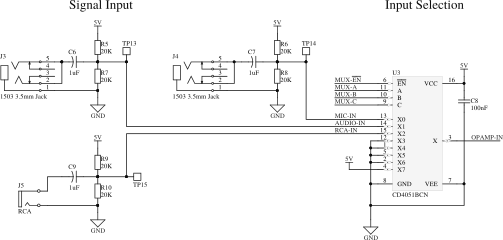
\includegraphics[width=.8\linewidth]{figures/circuits/input-selection.pdf}
    \caption{Circuito di selezione delle entrate \label{fig:input-selection}}
\end{figure}

Tutte le entrate dispongono di un condensatore di disaccoppiamento seguito da
un partitore di tensione simmetrico per aggiungere un offset della met\`a
dell'alimentazione. Il valore delle resistenze di 20\,k\(\Omega\) \`e scelto
per avere un impedenza rispetto al connettore pari all'impedenza
caratteristica dei cavi audio di 10\,k\(\Omega\).

\section{Circuito di entrata}
Il segnale di cui si analizza lo spettro, prima di essere campionato, viene
adattato mediate un circuito di amplificazione e filtraggio. Esso \`e
necessario per due ragioni. Il circuito di amplificazione \`e presente per
ovvie ragioni, quali per poter adattare il circuito nel caso in cui si dovesse
avere in entrata un segnale di ampiezza molto piccola. Il secondo circuito
invece, di filtraggio, \`e necessario per rimuovere disturbi di alta frequenza
che potrebbero compromettere la qualit\`a del campionamento. Questa \`e una
tipica configurazione prima di un circuito di conversione AD (analogico -
digitale), ed \`e conosciuto anche come circuito di filtraggio
\emph{anti-alias}.

\begin{figure}[H] \centering
    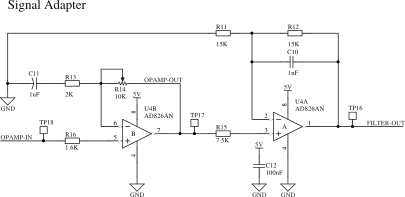
\includegraphics[width=.8\linewidth]{figures/circuits/filter-ampl.pdf}
    \caption[Circuito di adattamento del segnale]{
        Circuito di adattamento del segnale in entrata.
        \label{fig:filter-ampl}
    }
\end{figure}

\`E importante notare che per questa applicazione si \`e scelto utilizzare
degli opamp \emph{rail to rail}, che hanno una tensione di saturazione vicina
a quella di alimentazione. Essi sono necessari per poter raggiungere tensioni
vicino allo 0\,V, che non sarebbero possibili con un opamp normale siccome
l'alimentazione del circuito \`e asimmetrica tra 0 e 12\,V.

\paragraph{Amplificatore.} Come si pu\`o notare a sinistra nella figura
\ref{fig:filter-ampl}, il circuito di amplificazione non ha una configurazione
tipica. Esso \`e basato su una configurazione non invertente ma dispone di un
consensatore (C11) che modifica la retroazione in modo da reagire unicamente
alla componente AC del segnale. Questo permette di amplificare la componente
alternata ignorando l'offset del segnale, perci\`o di \emph{non} utilizzare
un'alimentazione simmetrica \(\pm\)5\,V.

L'amplificazione di questo amplificatore \`e comunque data dal rapporto
\(1+R_{14}/R_{13}\) che permette un un guadagno fino a 6 oppure 15,5\,dB.


\paragraph{Filtro.} A destra della figura \ref{fig:filter-ampl} vi \`e il
circuito di filtraggio, realizzato utilizzando un tipico filtro passa basso
attivo di primo ordine. Esso \`e dimensionato con una frequenza di taglio di
10\,kHz poich\`e quest'ultimo \`e il limite di Nyquist, conosciuto anche dal
teorema di Shannon, il quale stata che la frequenza di campionamento deve
essere almeno doppia della frequenza dell'armonica di frequenza maggiore.

Anche il filtro essendo non invertente ha un rapporto di amplificazione dato
da \(1+R_{12}/R_{11}\). Nella figura il valore della resistenza \(R_{11}\) \`e
\textbf{incorretto} (Vedi sezione \ref{sec:err-filter}). Dopo la correzzione
il filtro ha un amplificazione approssimativamente unitaria.

\section{Microcontroller}

\section{Visualizzazione}
